\section{Final Solution} \label{sec:final-solution}

The final solution for FANS is displayed in Figure \ref{fig:deployment}. This solution uses a distributed systems
approach to create a multi-node fire response system controlled via a web interface.

\subsection{Deployment Diagram}

The primary node in our FANS project is the sensor data collection node, which monitors temperature and smoke
concentration levels. All sensor measurements are written to the Firebase cloud database for display by the web UI.

When a measurement is detected above the user-defined threshold, the sensor data collection node sends a UDP message
signifying an emergency over the local network to the notification system and alarm system nodes. Upon receipt of this
message, the notification system will send emails and SMS notifications to all users in its local database. The alarm
system node will begin blinking an LED and sounding an alarm.

In addition to the UDP message, the sensor data collection node will raise an emergency flag in the Firebase database
which signifies to the UI and the wearable haptic alarm that an emergency is active. The haptic alarm wearable device
will then begin blinking an LED and buzzing until the user disables it or the emergency ends.

The UI provides an interface for checking on the status of an emergency and reviewing sensor data in real-time. Users
can disable the emergency response from the UI when the emergency has been resolved, and they can also time out the
system’s emergency response whenever the system is falsely triggered (smokey cooking). Finally, the UI also allows user
contact information to be added to the subscriber list for emergency notifications.

\begin{figure}
    \centering
    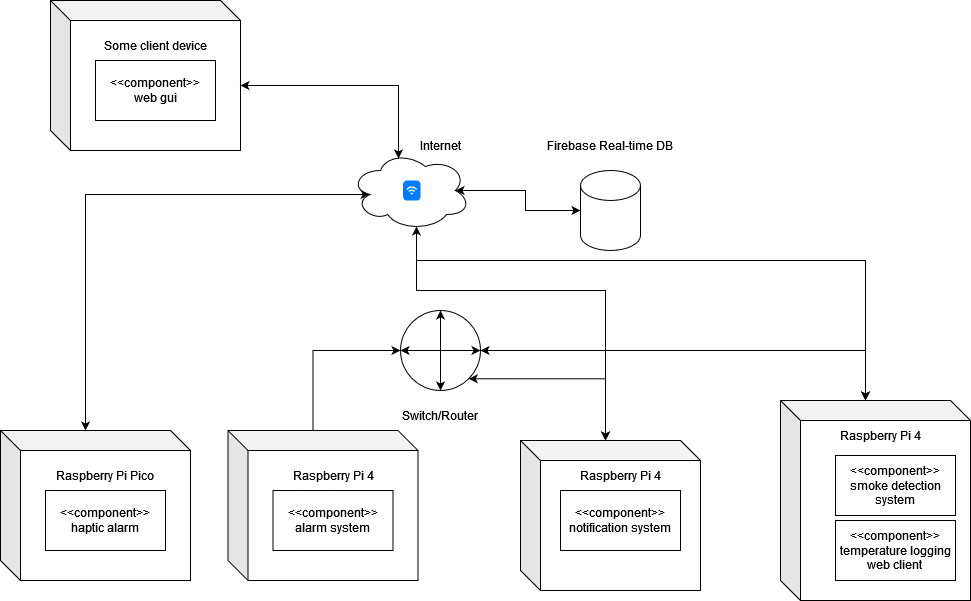
\includegraphics[width=\imagewidth]{../assets/FANSDeployment.png}
    \caption{The FANS deployment diagram.}
    \label{fig:deployment}
\end{figure}

\subsection{Message Protocol Table}

In the Fire Alarm Notification System (FANS), a variety of communication protocols are meticulously integrated to
ensure seamless interaction among the system components and with the external cloud database.

The system’s core, the Smoke Detection System, communicates with its temperature and smoke sensors using the I2C and
SPI protocols over the GPIO pins of a Raspberry Pi 4.

\subsubsection{I2C \& SPI Communication}

The Raspberry Pi 4 utilizes the I2C and SPI protocol to communicate with temperature and smoke sensors, monitoring
environmental conditions to detect potential fire hazards. These messages are outlined in \ref{table:i2c}.

\begin{table}
    \centering
    \begin{tabular}{| c | c | c | c | c |}
        \hline
        Sender         & Receiver               & Message              & Data Format                                          & Protocol                 \\
        \hline
        Raspberry Pi 4 & Temperature Sensor     & \texttt{read\_temp}  & See section 6.2.1 of datasheet \cite{temp-datasheet} & I2C                      \\
        \hline
        Raspberry Pi 4 & Smoke Sensor (via ADC) & \texttt{read\_smoke} & See figure 1.1 of datasheet \cite{adc-datasheet}     & SPI \cite{adc-datasheet} \\
        \hline
    \end{tabular}
    \caption{Messages for I2C communication in FANS.}
    \label{table:i2c}
\end{table}

\subsubsection{Local Area Network Communication}

Nodes within the FANS (smoke detection, alarm, and notification systems) communicate over a local network using UDP
packets, facilitating real-time alerts and system coordination. The messages sent over UDP use numerical value to
encode messages. The representation agreed upon is shown in Table \ref{table:udp-rep}. The messages sent are in Table
\ref{table:udp-messages}

\begin{table}
    \centering
    \begin{tabular}{| c | c |}
        \hline
        Message      & Value \\
        \hline
        Emergency    & 0     \\
        \hline
        No Emergency & 1     \\
        \hline
    \end{tabular}
    \caption{Numerical representation of messages over UDP in FANS.}
    \label{table:udp-rep}
\end{table}

\begin{table}
    \centering
    \begin{tabular}{| c | c | c | c | c |}
        \hline
        Sender                 & Receiver            & Message      & Data Format & Protocol \\
        \hline
        Smoke detection system & Notification system & Emergency    & 0           & UDP      \\
        \hline
        Smoke detection system & Alarm system        & Emergency    & 0           & UDP      \\
        \hline
        Smoke detection system & Notification system & No emergency & 1           & UDP      \\
        \hline
        Smoke detection system & Alarm system        & No Emergency & 1           & UDP      \\
        \hline
    \end{tabular}
    \caption{Messages for local area network communication in FANS.}
    \label{table:udp-messages}
\end{table}

\subsubsection{Cloud Database Communication}

Messages between each node and the Firebase database are shown in Table \ref{table:firebase}.

\begin{table}
    \centering
    \begin{tabular}{| c | c | c | c | c |}
        \hline
        Sender          & Receiver & Message                                    & Data Format                      & Protocol    \\
        \hline
        Smoke Detection & Cloud DB & \texttt{put\_sensor\_data()}               & See listing \ref{lst:sensor}     & HTTP (JSON) \\
        \hline
        GUI             & Cloud DB & \texttt{update\_threshold(new\_threshold)} & See listing \ref{lst:threshold}  & HTTP (JSON) \\
        \hline
        Notification    & Cloud DB & \texttt{query\_contact\_information()}     & See listing \ref{lst:contact}    & HTTP (JSON) \\
        \hline
        Haptic Alarm    & Cloud DB & \texttt{emergency()}                       & See listing \ref{lst:emergency}  & HTTP (JSON) \\
        \hline
        GUI             & Cloud DB & \texttt{get\_sensor\_data()}               & See listing \ref{lst:sensor-get} & HTTP (JSON) \\
        \hline
    \end{tabular}
    \caption{Messages for cloud database communication in FANS.}
    \label{table:firebase}
\end{table}

{
\tiny
\begin{lstlisting}[language=json,label={lst:sensor},caption={Update sensor data message.}]
{
  "method": "PUT",
  "path": "/sensor-data/temperature",
  "headers": {
    "Authorization": "Bearer YOUR_ACCESS_TOKEN",
    "Content-Type": "application/json"
  },
  "body": {
      "data": {
          "temperature": 21.2,
          "timestamp": "2024-03-13T08:37:22"
      }
  }
}
\end{lstlisting}

\begin{lstlisting}[language=json,label={lst:threshold},caption={Threshold update message.}]
{
  "method": "PUT",
  "path": "/system/threshold",
  "headers": {
    "Authorization": "Bearer YOUR_ACCESS_TOKEN",
    "Content-Type": "application/json"
  },
  "body": {
    "newThreshold": 50
  }
}
\end{lstlisting}

\begin{lstlisting}[language=json,label={lst:contact},caption={Request for user contact information.}]
{
  "method": "GET",
  "path": "/user/contact",
  "headers": {
    "Authorization": "Bearer YOUR_ACCESS_TOKEN"
  }
}
\end{lstlisting}

\begin{lstlisting}[language=json,label={lst:emergency},caption={Request for emergency flag.}]
{
  "method": "GET",
  "path": "/system/emergency",
  "headers": {
    "Authorization": "Bearer YOUR_ACCESS_TOKEN"
  }
}
\end{lstlisting}

\begin{lstlisting}[language=json,label={lst:sensor-get},caption={Request for latest sensor data.}]
{
  "method": "GET",
  "path": "/sensor-data",
  "headers": {
    "Authorization": "Bearer YOUR_ACCESS_TOKEN"
  }
}
\end{lstlisting}
}

\subsubsection{User Notification Communication}

The notification system communicates with users through email, employing standard internet protocols to ensure timely
and effective alerts.

\begin{table}[H]
    \centering
    \begin{tabular}{| c | c | c | c | c |}
        \hline
        Sender              & Receiver   & Message                & Data Format                 & Protocol     \\
        \hline
        Notification System & User Inbox & Emergency notification & See listing \ref{lst:email} & SMTP (Email) \\
        \hline
    \end{tabular}
    \caption{Messages for user notification communication in FANS.}
\end{table}

{
\tiny
\begin{lstlisting}[label={lst:email},caption={Email notification for detected emergency in FANS.}]
FROM: notification@example.com
TO: user@example.com
SUBJECT: Fire Alarm Notification

Dear [User's Name],

This is an emergency notification. Please exit the building.

Emergency detected: [Date, Time]

Stay safe!
\end{lstlisting}
}

\subsection{Sequence Diagrams}

The FANS system satisfies several core use cases. The three most critical use cases are shown below, and more detail
can be found in Appendix \ref{ap:sequence}.

\subsubsection{Trigger Emergency Use Case}

The trigger emergency use case shown in Figure \ref{fig:trigger-emerg} describes the critical functionality of FANS,
where the system detects a potential fire and initiates a series of automated responses to mitigate the situation. As
depicted in Figure \ref{fig:trigger-emerg}, the process begins when the smoke detection system identifies smoke and
potentially high temperatures indicative of a fire. This detection triggers a UDP notification to the alarm and
notification systems to alert them to begin their automated emergency responses. It additionally raises a flag in the
Firebase cloud database for non-local nodes (such as the haptic alarm) to begin their responses.

\begin{figure}
    \centering
    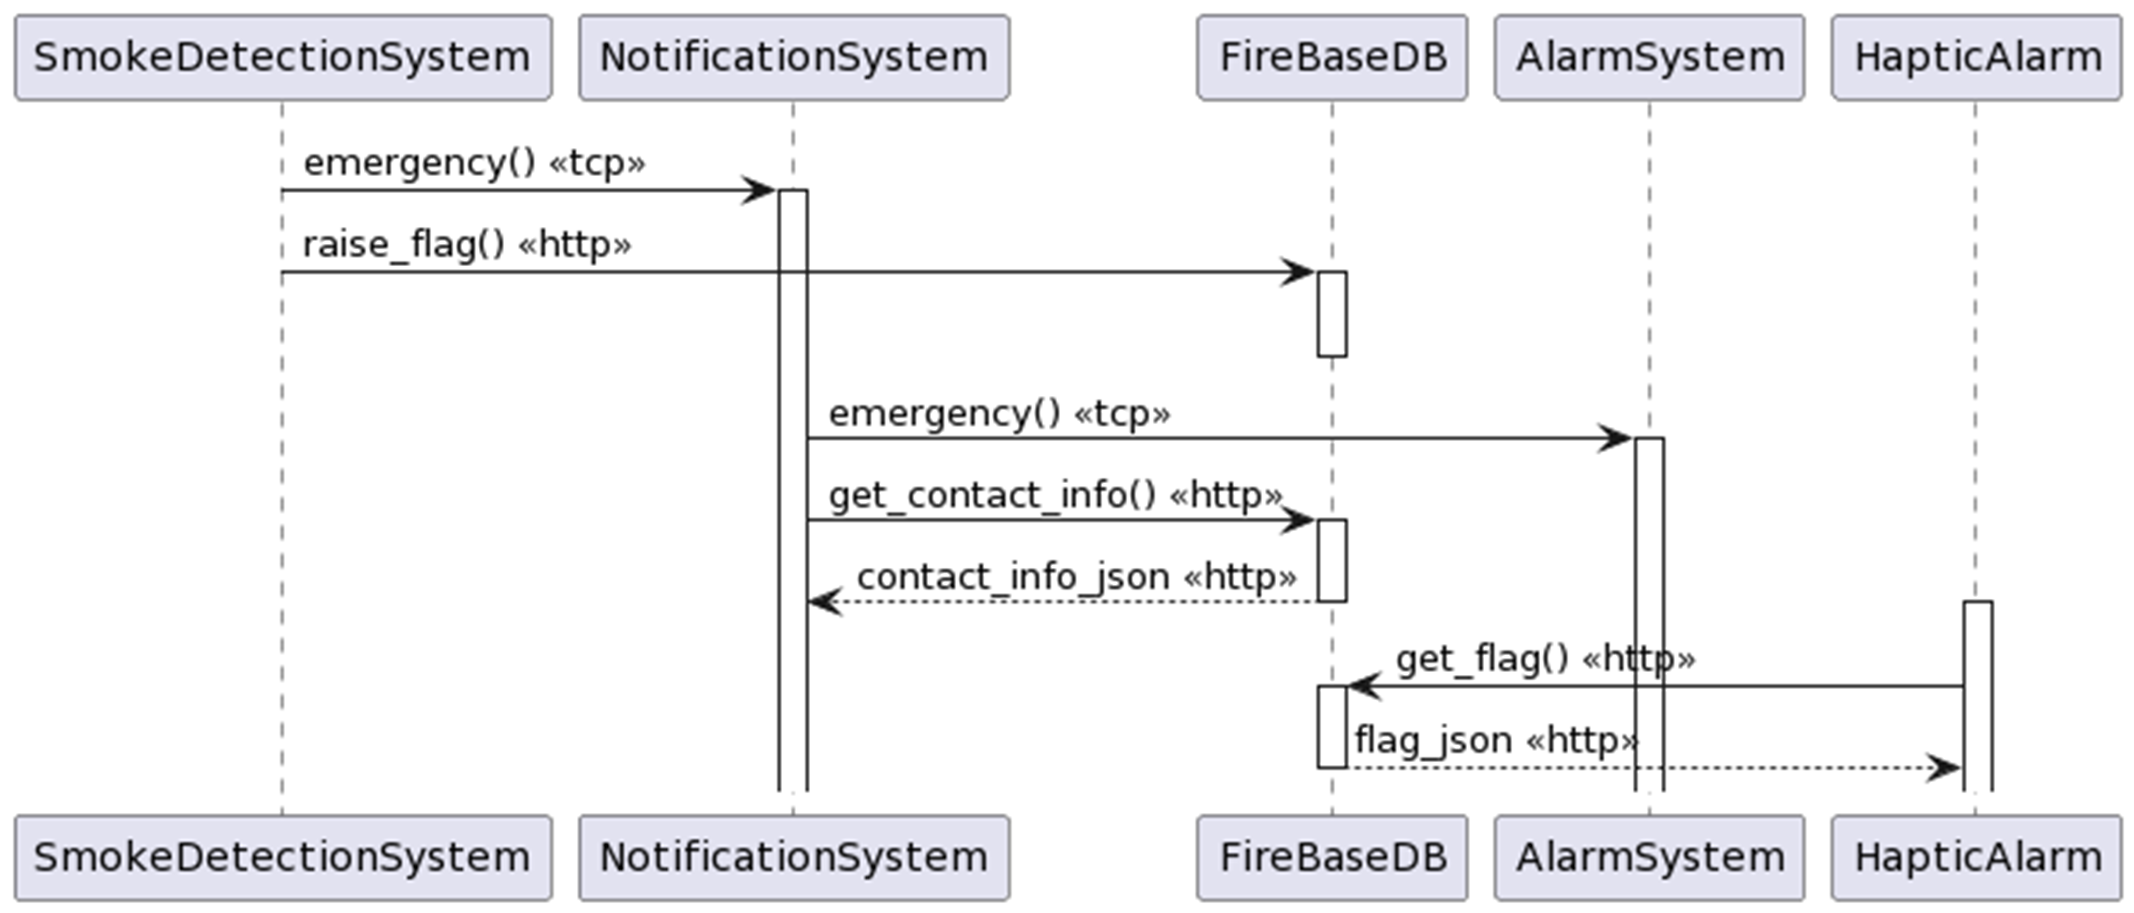
\includegraphics[width=\imagewidth]{../assets/sequence/TriggerEmergencyUseCaseSequenceDiagram.png}
    \caption{The sequence diagram for the trigger emergency use case.}
    \label{fig:trigger-emerg}
\end{figure}

\subsubsection{Change Emergency Threshold Use Case}

Adjusting the smoke detection threshold is an essential feature that allows users to customize the sensitivity of the
FANS based on personal and environmental conditions. This use case, shown in Figure \ref{fig:change-thresh}, involves a
user accessing the web GUI to modify the threshold settings. Once the user submits their new thresholds, the web GUI
sends an update request to the database and displays a confirmation to the user. The smoke detector unit periodically
checks the thresholds in the database for updates, and updates its local values when it detects a change.

\begin{figure}
    \centering
    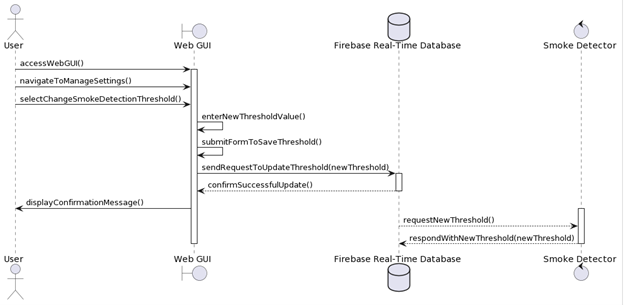
\includegraphics[width=\imagewidth]{../assets/sequence/ChangingSmokeDetectionThresholdSequenceDiagram.png}
    \caption{The sequence diagram for the changing emergency threshold use case.}
    \label{fig:change-thresh}
\end{figure}

\subsubsection{Emergency Notification Use Case}

The scenario in Figure \ref{fig:emergency-resp} highlights FANS capability to notify users in the event of a detected
fire. Upon being notified of an emergency, the notification system queries the cloud database for contact information
and sends out alerts via SMS and email to all users. If the cloud database is not accessible, the local database is
instead used.

\begin{figure}
    \centering
    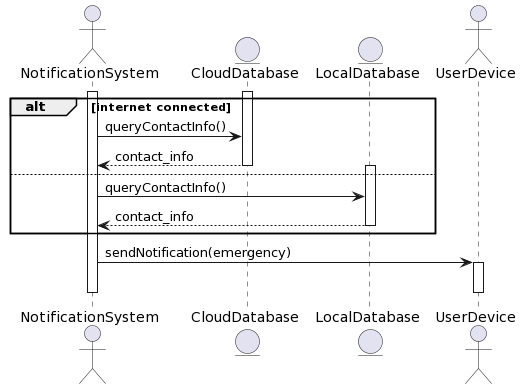
\includegraphics[width=3in]{../assets/sequence/EmergencyResponseUseCase.png}
    \caption{The sequence diagram for the emergency notification use case.}
    \label{fig:emergency-resp}
\end{figure}
